\documentclass[mathserif]{beamer}
\usetheme[secheader]{pecostalk}
\graphicspath{{figs/}}                                                                                                                              


\date{December 7, 2014}
\author[A. W. Fullname]{Author W. Fullname}
\institute{The University of Texas at Austin}
\title[Short Title]{Long Title of This Talk}
\subtitle{With A Subtitle If Necessary}

\begin{document}
\begin{frame}
\begin{center}
\end{center}
\titlepage
\begin{flushright}
\end{flushright}
\end{frame}

%===============================================================================
% NEW SLIDE
%===============================================================================
\begin{frame}
\frametitle{Your 10-15 minute presentation will have \ldots}

\begin{itemize}
\item 2 slides on intro to the problem
\item what feature you're adding if appropriate
\item build system and version control infos
\item Verification plan
\item Convergence plots
\item Grvy timer results or something similar
\item Code coverage (if appropriate)
\item How did you start out?
\begin{itemize}
\item What worked?
\item What didn't work?
\end{itemize}
\item If you were starting over \ldots
\begin{itemize}
\item What would you do differently?
\item What would you do the same?
\end{itemize}
\item Lessons learned
\end{itemize}

\end{frame}

%===============================================================================
% NEW SLIDE
%===============================================================================
\begin{frame}
\frametitle{Basic Slide}

This is a basic slide. There are many like it, but this one is mine.
\begin{itemize}
\item item 1
\item item 2
\item item 3
\item item 4
\end{itemize}

\end{frame}

%===============================================================================
% NEW SLIDE
%===============================================================================
\begin{frame}
\frametitle{Example 1: 2 Blocks with nested item lists}
%===============================
\begin{block}{First Block}
\begin{itemize}
\item First Item
	\begin{itemize}
	\item Subitem
	\end{itemize}
\item Second Item:
	\begin{itemize}
	\item More subitems
	\item And more
	\end{itemize}
\end{itemize}
\end{block}
%===============================
\begin{block}{Second Block}
\begin{itemize}
\item With an item
\end{itemize}
\end{block}
%===============================
\end{frame}






%===============================================================================
% NEW SLIDE
%===============================================================================
\begin{frame}
\frametitle{Example 2: 2 Columns;\\ one column with two blocks, one block with two columns!}
\begin{columns}[c]
\begin{column}{5cm}
\begin{block}{Block 1}
\begin{columns}[t]
\begin{column}{2.25cm}
\begin{itemize}
\item item 1\\
\item item 2\\
\item item 3\\
\end{itemize}
\end{column}
\begin{column}{2.75cm}
\begin{itemize}
\item item 4\\
\item item 5\\
\item item 6\\
\end{itemize}
\end{column}
\end{columns}
\end{block}
\begin{block}{Block 2}
\begin{itemize}
\item item A\\
\item item B\\
\end{itemize}
\end{block}
\end{column}
\begin{column}{5cm}
\begin{block}{Block 3}
\begin{itemize}
\item item a\\
\item item b\\
\item item c\\
\item item d\\
\end{itemize}
\end{block}
\end{column}
\end{columns}
\end{frame}
%===============================================================================
% NEW SLIDE
%===============================================================================
\begin{frame}                                                                                                                                                                          
\frametitle{Image and Bullet points}
\begin{center}
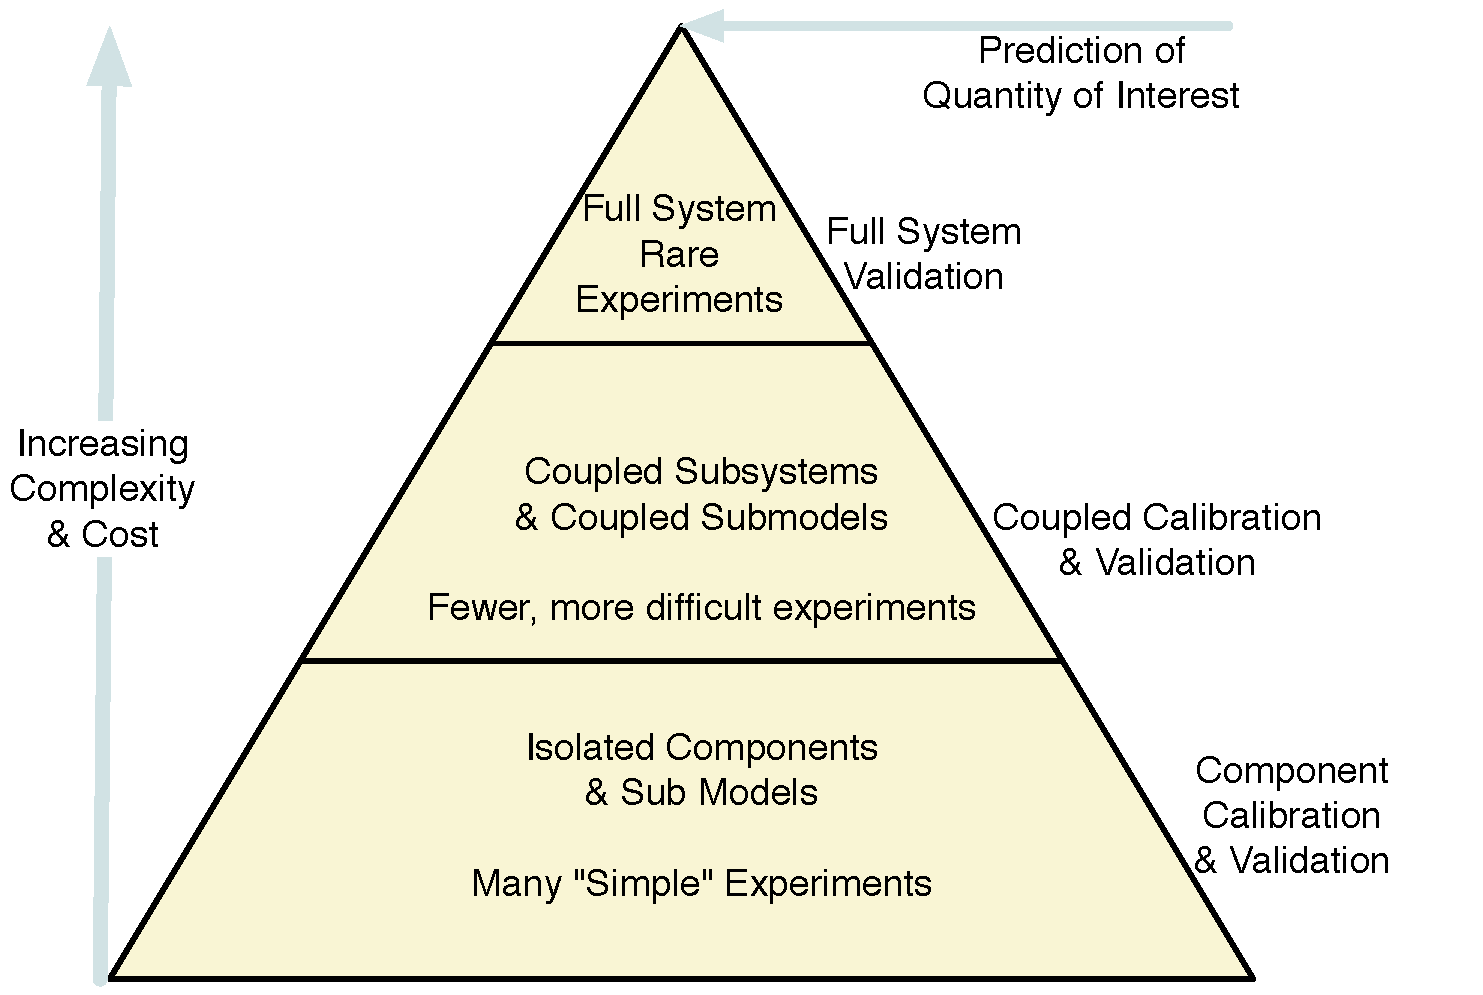
\includegraphics[width=.8\linewidth]{generic_pyramid}\\
\begin{itemize}
\item Validation is done repeatedly with increasingly complex scenarios
\item Validation pyramid may be recursive
\end{itemize}
\end{center}
\end{frame}              
%===============================================================================
% NEW SLIDE
%===============================================================================
\begin{frame}
\frametitle{Two Blocks with added text for emphasis}

{\color{pecos2}V\&V-UQ framework \emph{requires} experimental data}
\begin{block}{Calibration of component model parameters}
\begin{itemize}
\item Thermochemistry (e.g. kinetic parameters)
\item Radiation (e.g. absorptions \& emissions)
\item Turbulence (e.g. model constants)
\item Ablation (e.g. kinetic parameters)
\end{itemize}
\end{block}
\begin{block}{Validation}
\begin{itemize}
\item Component and subcomponent models
\item Coupling between models
\item Full system
\end{itemize}
\end{block}
\end{frame}

%===============================================================================
% NEW SLIDE
%===============================================================================
\begin{frame}                                                                                                                                                                          
\frametitle{1 Block and 1 Image in Column format}
\begin{columns}[c]
\begin{column}{5cm}
\begin{block}{Extensive experimental data}
\begin{itemize}
\item {\color{pecos6}Space Act Agreement}
\begin{itemize}
\item Ames EAST
\item Langley RCS
\item Ames \& JSC Arc Jets
\item AEDC T9
\item CUBRC
\item Cal Tech
\end{itemize}
\item Legacy data
\item Sandia
\item PECOS
\end{itemize}
\end{block}
\end{column}
\begin{column}{5cm}
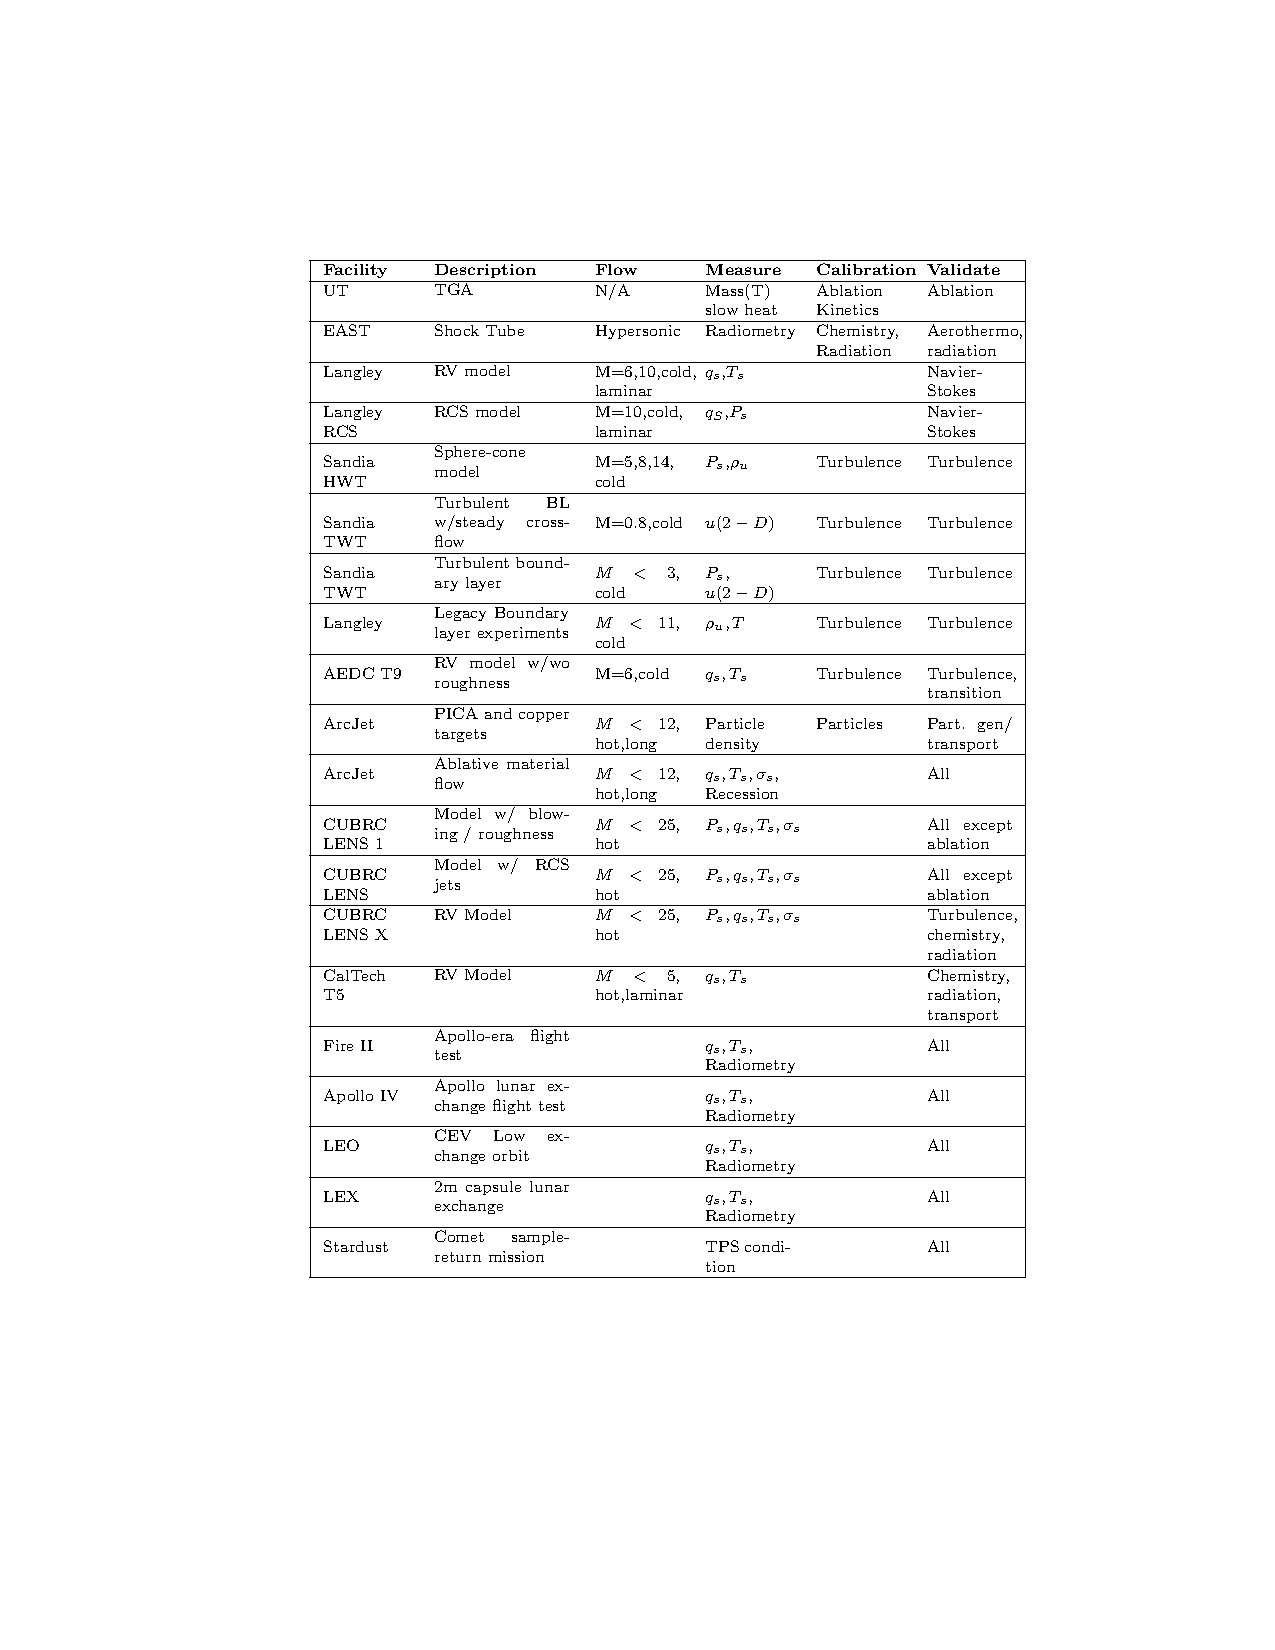
\includegraphics[scale=0.45]{validation_table}
\end{column}
\end{columns}
\end{frame}

%===============================================================================
% NEW SLIDE
%===============================================================================
\begin{frame}                                                                                                                                                                          
\frametitle{1 image and 1 itemized Block}
\begin{center}
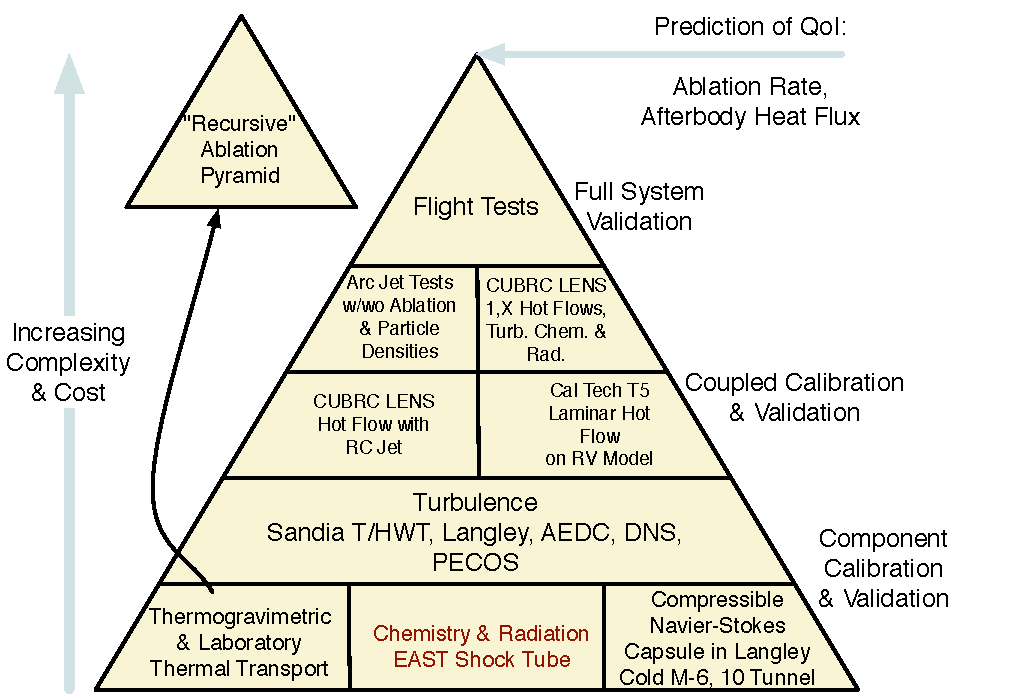
\includegraphics[width=.5\linewidth]{pyramid_east}\\
\end{center}
\begin{block}{Goals}
\begin{itemize}
\item Calibrate and (in)validate a two-temperature thermochemical model  
\item Investigate implementation of the validation cycle with QUESO  %
\item Develop a 1D problem for future exploration of adjoints
\end{itemize}
\end{block}
\end{frame}

%===============================================================================
% NEW SLIDE
%===============================================================================
\begin{frame}                                                                                                                                                                          
\frametitle{Block and then Two Images in a Column}
\vspace {-1 mm}
\begin{block}{Facility}
\begin{itemize}
\item LENS I HST
  \begin{itemize}
  \item Variable Re reflected shock tunnel
  \item Tests: Perfect gas data, enthalpy effects, distributed roughness, roughness w/ blowing,  high-fidelity
  \end{itemize}
\item LENS XX
  \begin{itemize}
  \item Variable Re shock expansion tunnel
  \item Tests: Facility and measurement capabilities similar to EAST
  \end{itemize}
\item Visit planned for May 2009
\end{itemize}
\end{block}

\begin{columns}
  \begin{column}[l]{0.45\linewidth}
  \begin{figure}[h]
  \begin{center}
  \vspace {-5 mm}
  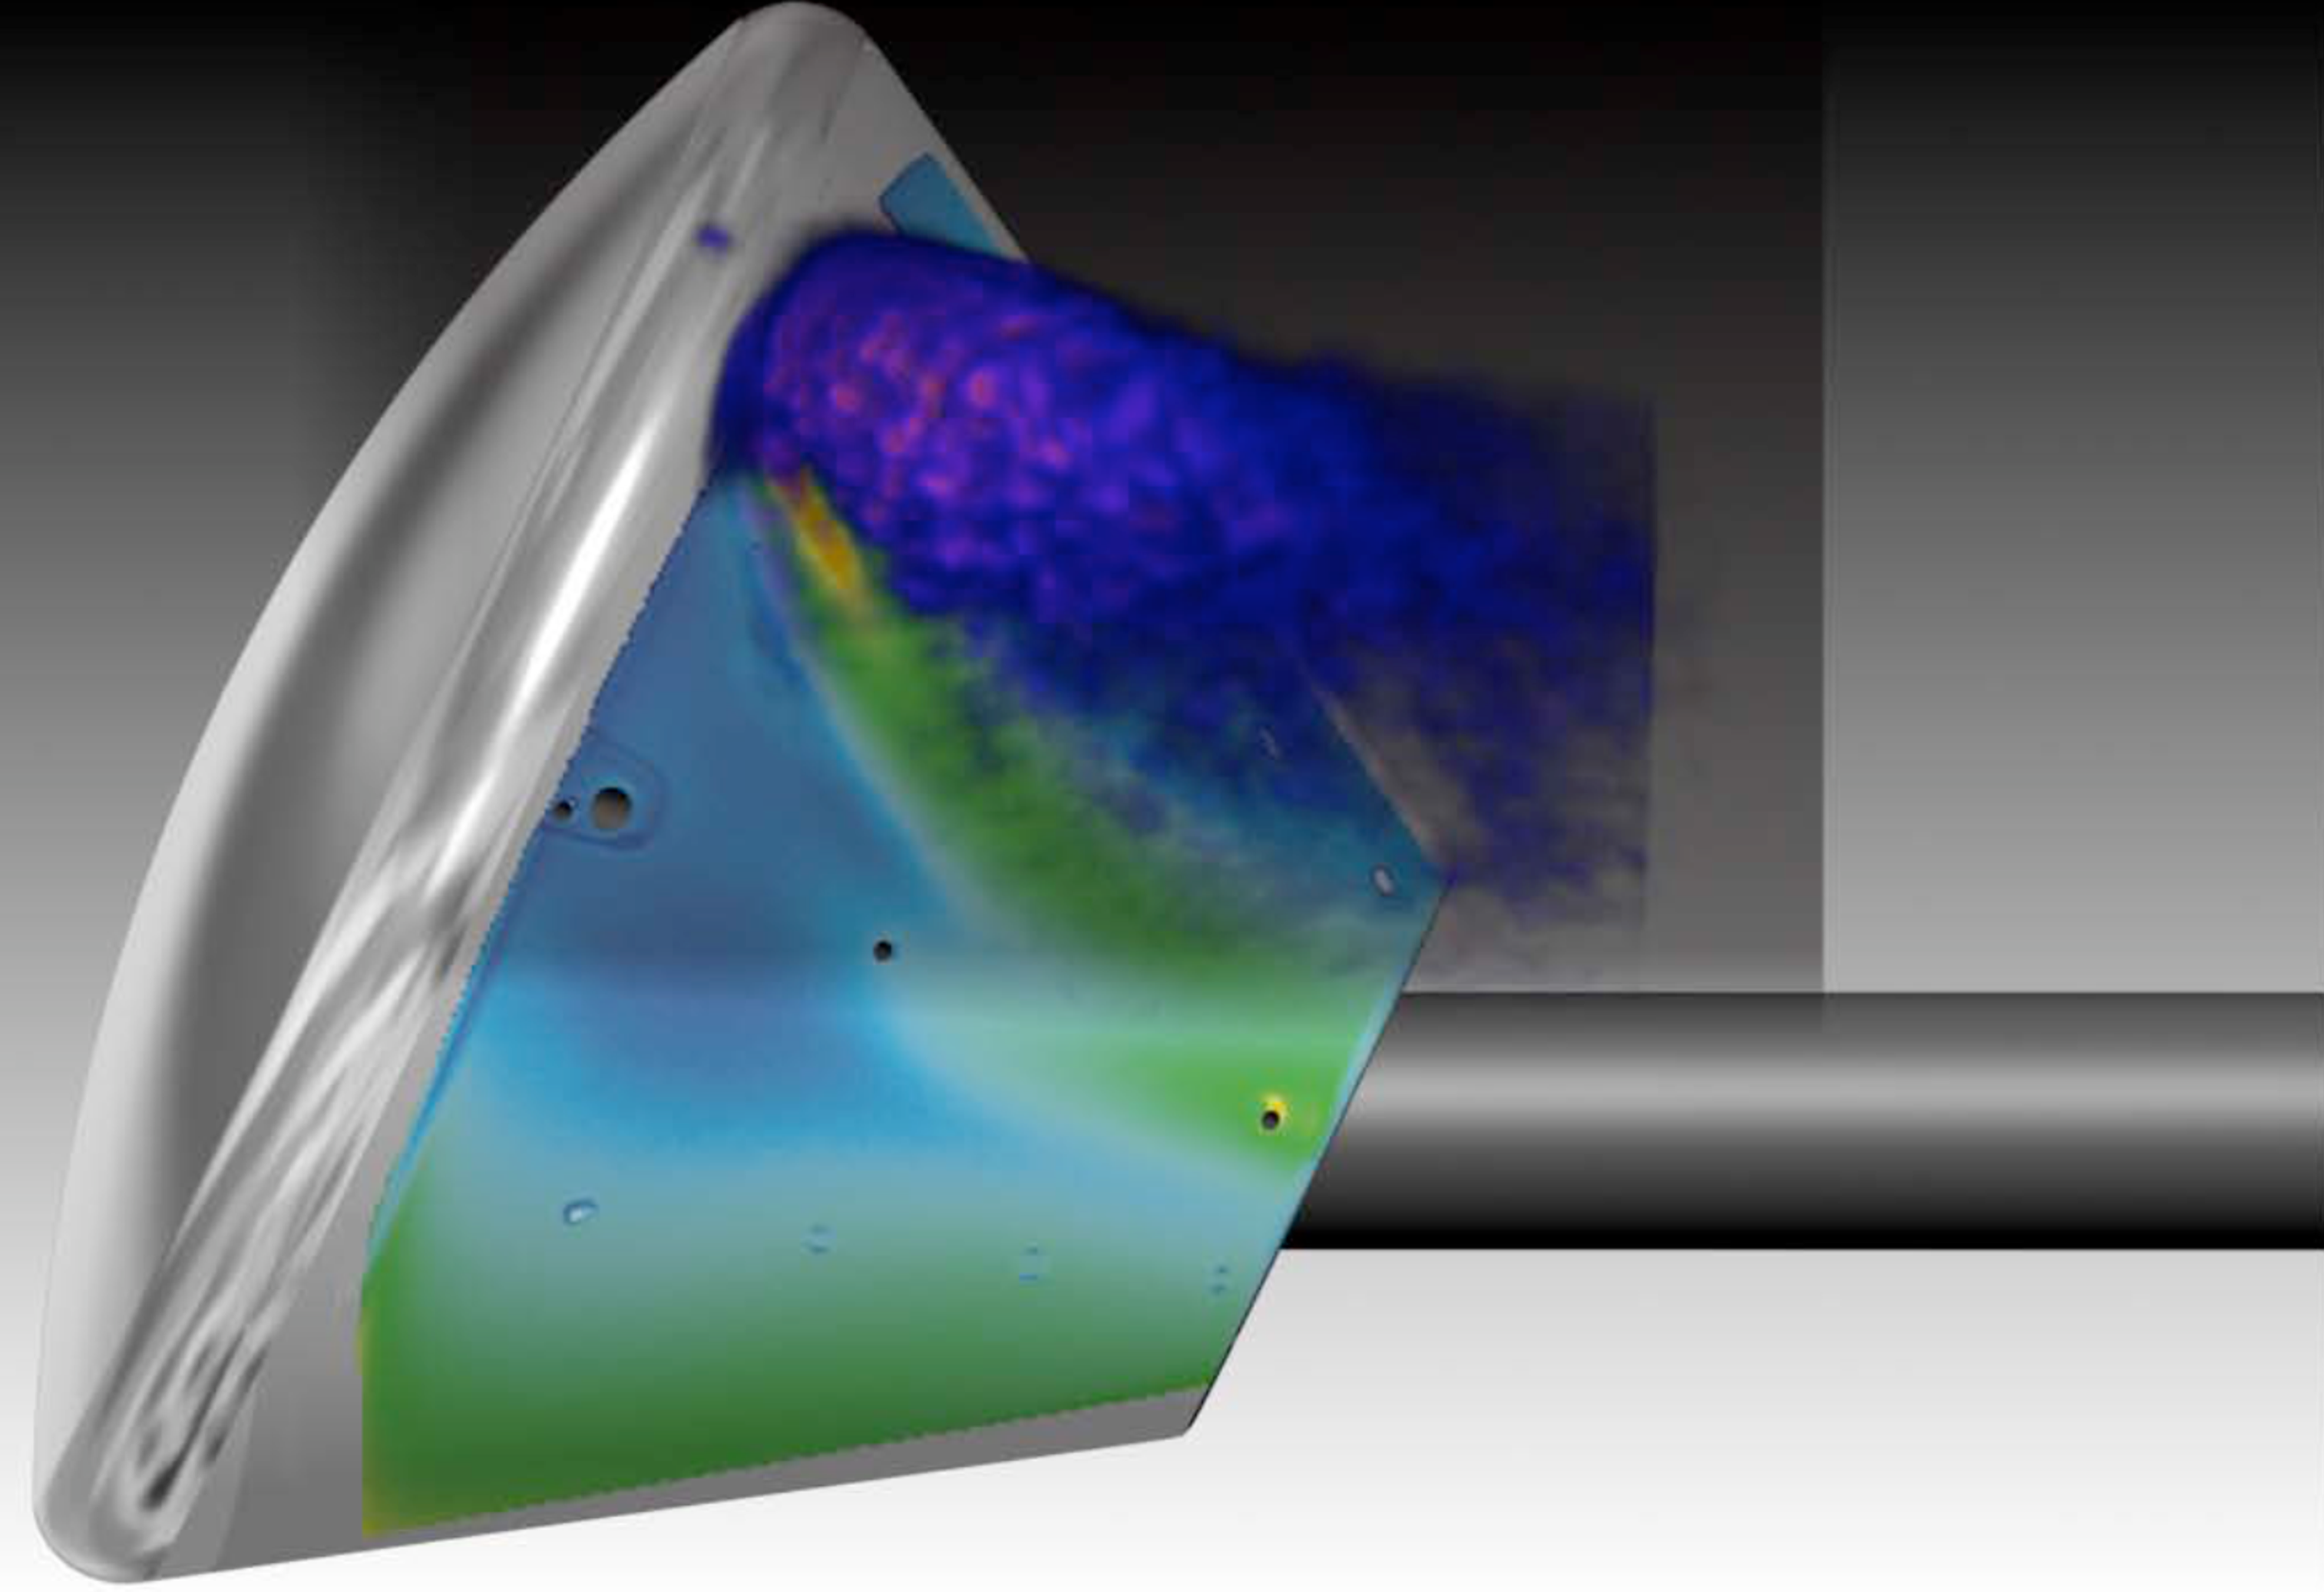
\includegraphics[width=0.9\linewidth]{RCS_PLIF.pdf} %This figure shows an RCS jet experiment at LaRC; low enthalpy vs. high enthalpy at CUBRC
  \end{center}
  \end{figure}
  \end{column}

  \begin{column}[r]{0.45\linewidth}
  \begin{figure}[h]
  \begin{center}
  \vspace {-5 mm}
  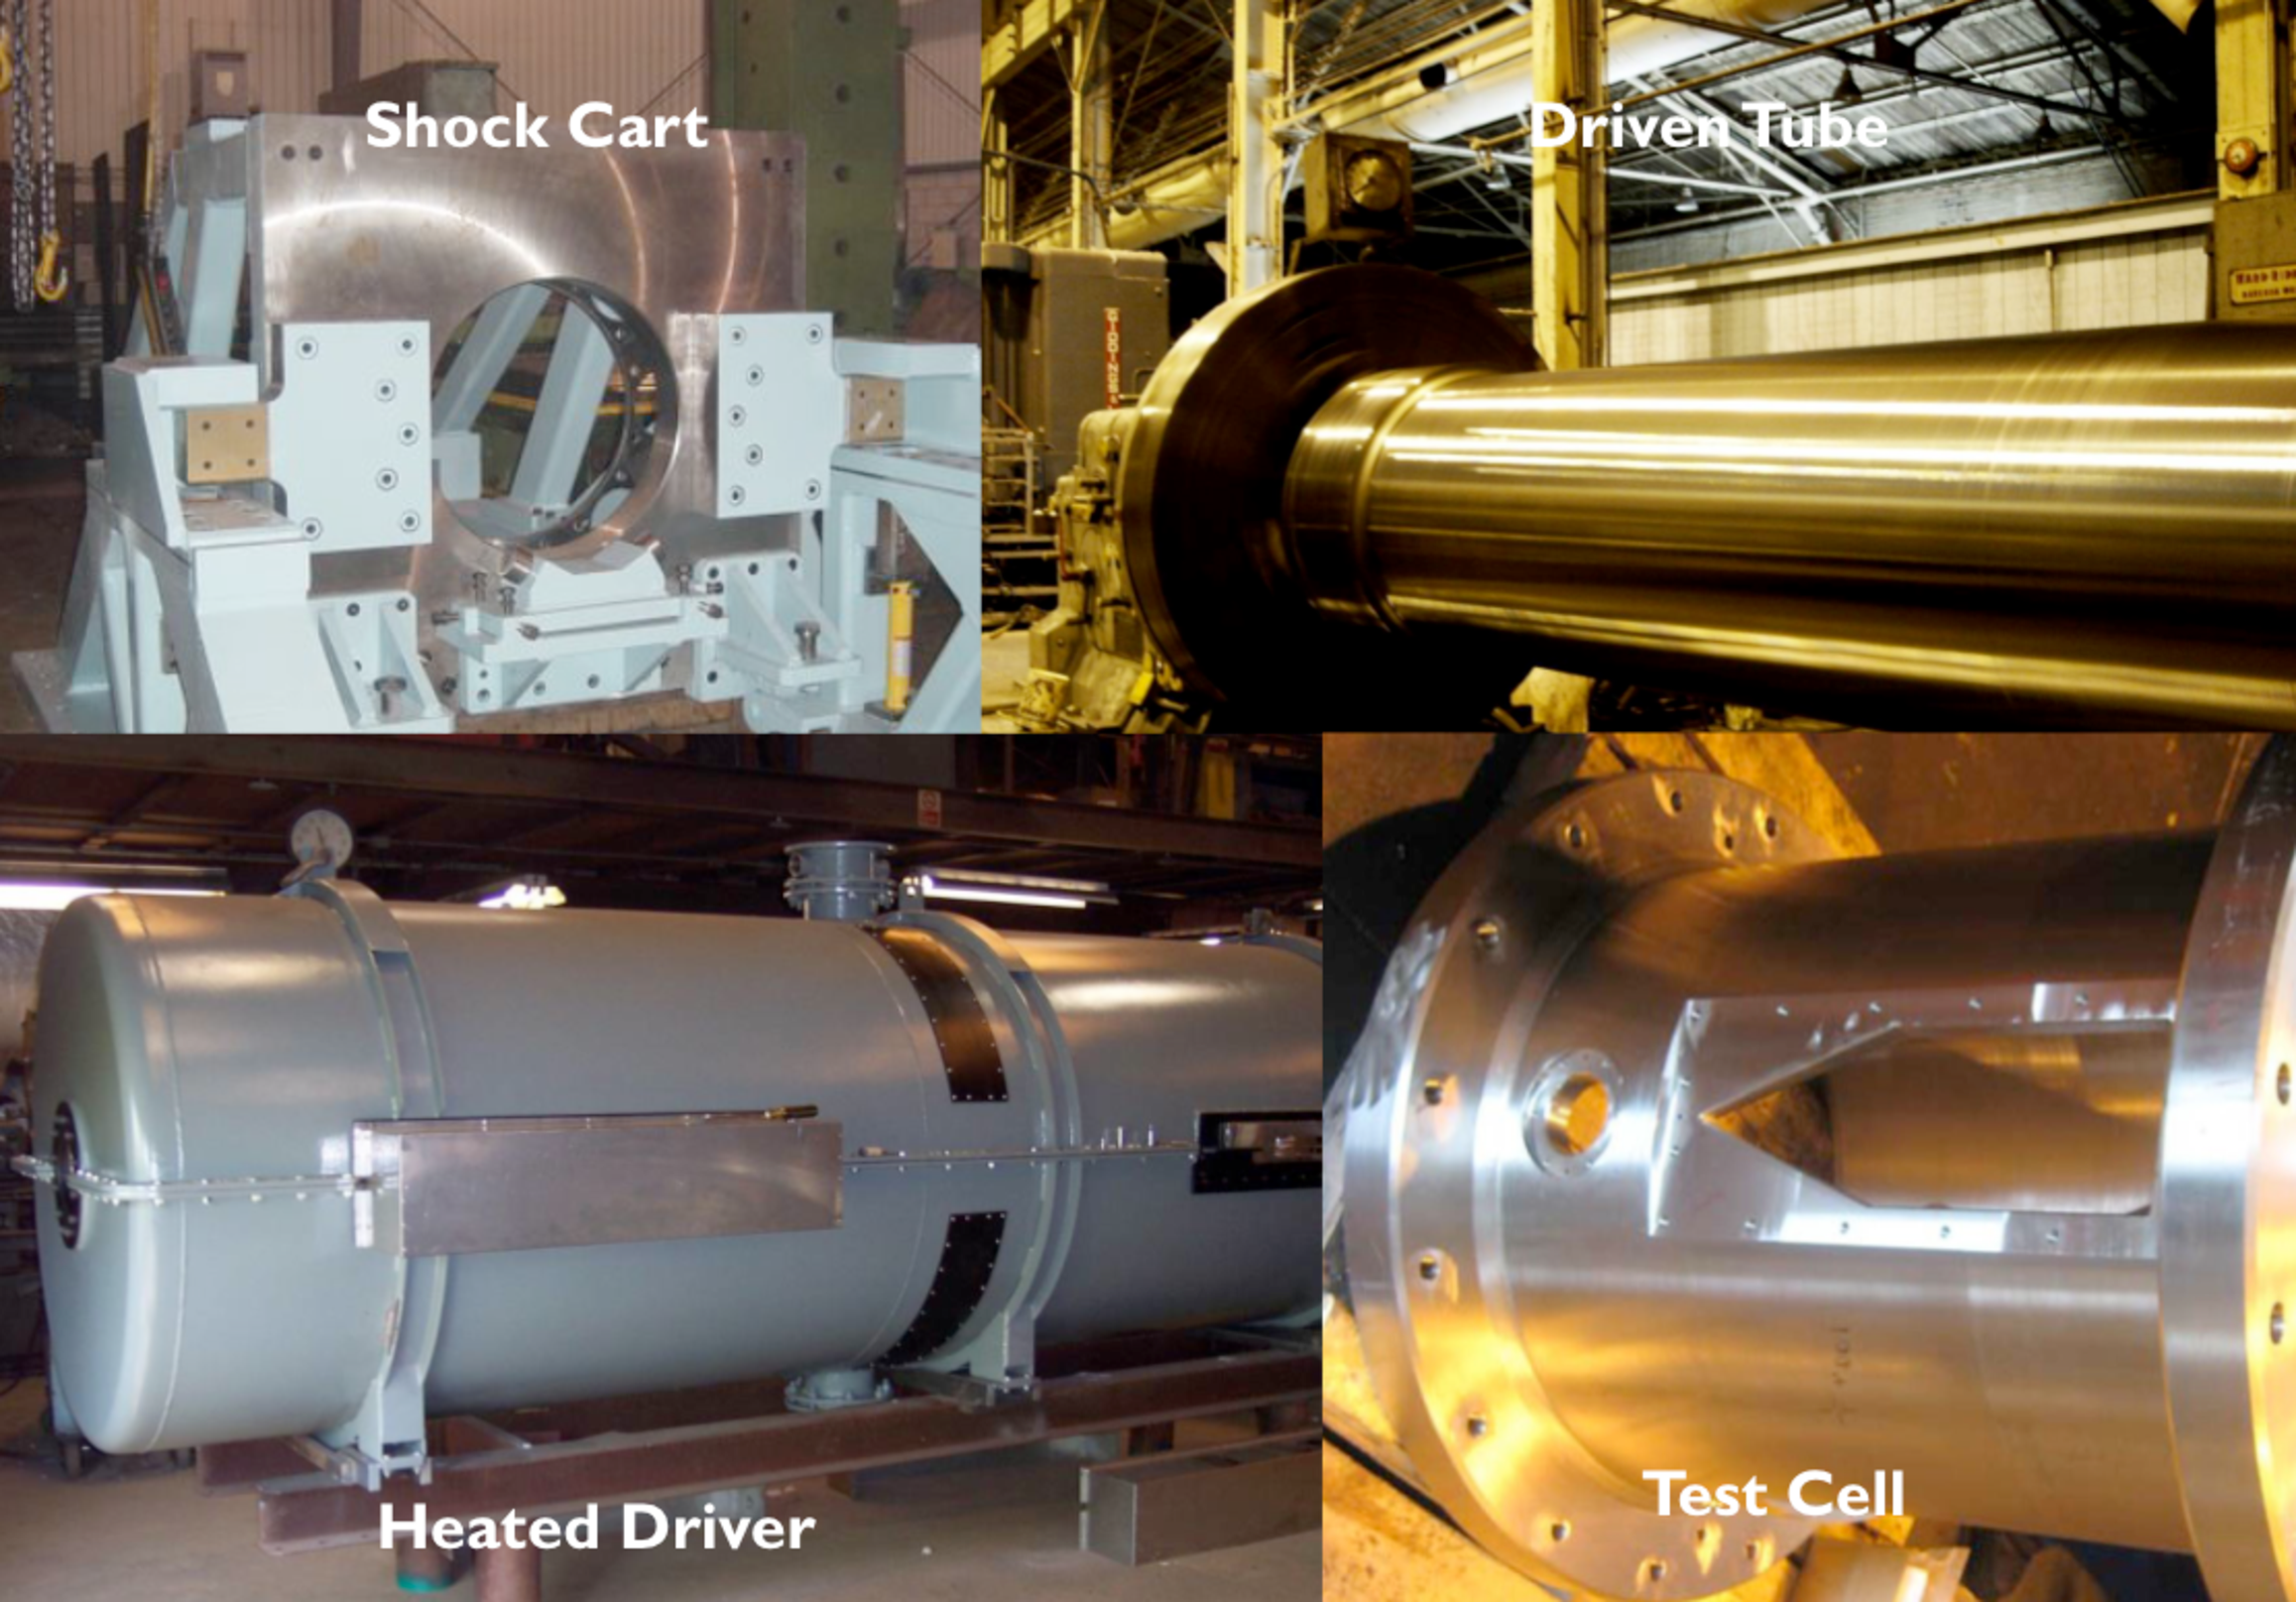
\includegraphics[width=0.9\linewidth]{LENSXX_components.pdf} %This figure shows some components of the new LENS XX facility
  \end{center}
  \end{figure}
  \end{column}
\end{columns}
\end{frame}

%===============================================================================
% NEW SLIDE
%===============================================================================
\begin{frame}
\frametitle{Two Images in Two Blocks in a Column}
\begin{columns}[c]
\begin{column}{5.5cm}
\begin{block}{Surface Ablation Rate}
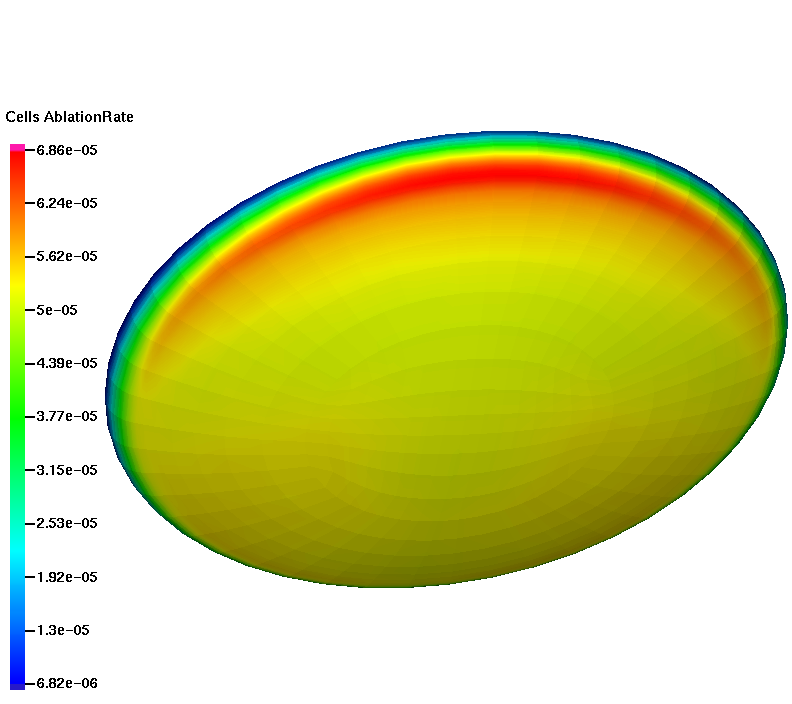
\includegraphics[width=5.5cm]{surface_ablation_rate_node_valued_coarse_mesh.png}
\end{block}
\end{column}
\begin{column}{5.5cm}
\begin{block}{Surface Heat Flux}
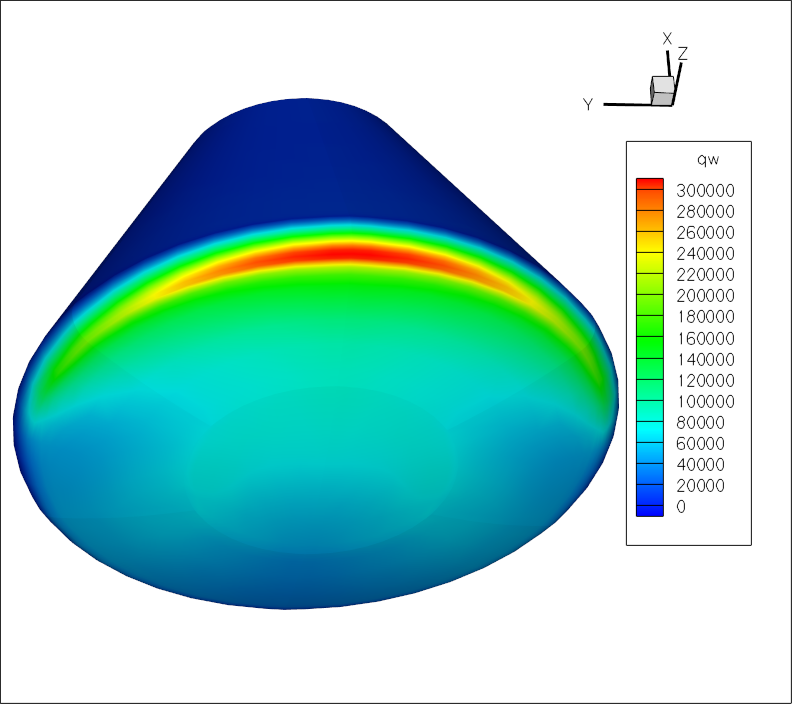
\includegraphics[width=5.5cm]{surface_heat_flux_coarse_mesh.png}
\end{block}
\end{column}
\end{columns}
\end{frame}


%===============================================================================
% NEW SLIDE
%===============================================================================
\begin{frame}                                                                                                                                                                          
\frametitle{Fancy Block / Column work}
\begin{block}{Goals}
\begin{itemize}
\item Demonstrate capability to couple ablation and radiation models with
existing hypersonic code (DPLR)
\item Evaluate sensitivity of the ablation rate and peak heat flux (QoIs)
\begin{itemize}
\item Identify most important models
\item Evaluate utility of surrogate quantities of interest
\end{itemize}
\end{itemize}
\end{block}
\begin{block}{Coupled hypersonic flow for LEO and lunar reentry, including:}
\begin{footnotesize}
\begin{columns}[T]
\begin{column}{5cm}
\begin{itemize}
\item Arrhenius chemistry
\item Gray temperature dependent radiation
\item Algebraic(Baldwin-Lomax) turbulence models
\end{itemize}
\end{column}
\begin{column}{5cm}
\begin{itemize}
\item Thermal nonequilibrium
\item Single phase flow (i.e. no particles)
\end{itemize}
\end{column}
\end{columns}
\begin{itemize}
\item 1-dimensional solid-phase ablation with ad hoc kinetics (as in CMA, FIAT, Chaleur)
\item Equilibrium surface chemistry
\end{itemize}
\end{footnotesize}
\end{block}
\end{frame}


%===============================================================================
% NEW SLIDE
%===============================================================================
\begin{frame}
\frametitle{}
\begin{block}{}
\center{Thank you!} \\
\center{Questions?}
\end{block}
\end{frame}

 
\end{document}
